\documentclass{report}
\usepackage{ctex}
\usepackage{xeCJK}

% 下划线宏包
\usepackage[normalem]{ulem}

% 绘图
\usepackage{tikz}
\usepackage{tikz-3dplot}
\usetikzlibrary{calc,intersections,positioning,angles,quotes,decorations.pathmorphing,fit,backgrounds,through,svg.path,topaths,patterns}

% \newcommand{cmd}[args][default]{def}
\newcommand{\tikzline}[1]{{#1\tikz{\draw[#1,line width=9](0,0)--(0.5,0);}}, }
\tikzset{math3d/.style={x={(-0.353cm,-0.353cm)},z={(0cm,1cm)},y={(1cm,0cm)}}}
\usetikzlibrary{calc,3d}

\usepackage{url}
\usepackage[colorlinks,linkcolor=blue]{hyperref}
 
\usepackage{fullpage}
\usepackage{fourier}

\usepackage{xcolor}  	%高亮使用的颜色
\usepackage{color}

% 数学环境
\usepackage{amsmath}
\usepackage{amsfonts}
\usepackage{amssymb}
\usepackage{mathdots} % 数学省略号,会重定义 dddot 和 ddddot
\newcommand{\ue}{\mathrm{e}}
\newcommand{\ud}{\mathop{}\negthinspace\mathrm{d}} % 微分号
\usepackage{mathrsfs} % 线性代数字体

% 奇怪的小定义
\newcommand{\dpar}{\\ \mbox{}}  % 空两行
\newcommand{\qd}[1]{{\bfseries{#1}}}  % 强调
\newcommand{\co}[1]{{\bfseries{#1}}}  % Style of concept
\newcommand{\RED}[1]{{\color{cyan}{#1}}}
\newcommand{\cmmd}[1]{\fbox{\texttt{\char92{}#1}}}
\newcommand{\charef}[1]{第\ref{#1}章}
\newcommand{\secref}[1]{第\ \ref{#1}\ 节}
\newcommand{\pref}[1]{第\pageref{#1}页}
\newcommand{\fref}[1]{图\ref{#1}}
\newcommand{\tref}[1]{表\ref{#1}}

% 页面修正宏包
\usepackage{geometry}
\geometry{vmargin = 1in}

\usepackage{listings}

\title{\LaTeX{} Review}
\author{Lin Guo}
\date{Begin:\ May 20, 2021}

\begin{document}

\maketitle
\tableofcontents

\part{\LaTeXe}

\chapter{\LaTeX{} 基础}

参考材料:\footnote{主要参考吴康隆《简单粗暴\LaTeX》}

\section{常用命令说明}


\begin{verbatim}
\emph{} %正/斜字体强调
\parindent % 行距?
\par %分段,带缩进
\mbox{} %空箱子,可占位
\hspace{len}
\vspace{len}
\newpage命令开始新的一页.
\clearpage命令清空浮动体队列5,并开始新的一页.
\cleardoublepage命令清空浮动体队列,并在偶数页上开始新的一页.
如果要连续新开两页,请在中间加上一个空的箱子(\mbox{}),如\newpage\mbox{}\newpage.

\end{verbatim}
\textbackslash dpar:

\section{目录}


\section{抄录与代码环境}

参考材料:\footnote{3.11节}

\section{\LaTeX{} 进阶}

\section{自定义环境与命令}
\begin{verbatim}
\newcommand{cmd}[args][default]{def} % 类似于函数:函数名;参数;默认参数;定义
\renewcommand{cmd}[args][default]{def}
\newenvironment{name}[args][default]{begdef}{enddef}
% 示例见导言区
\end{verbatim}

例,\qd{强调}



参考材料:\footnote{5.1节}

\section{自定义章节样式}


\chapter{Structure of source files}

\chapter{Commands}
\section{高亮}
Learn later. Not need NOW!
\subsection{使用verbatim环境}
抄录命令与抄录环境。

verbatim 环境可以原样输出其中的文本,忽略TeX命令。

对简短的抄录,可使用 。
\subsection{其他?}
- listings

%\begin{shaded}
%\begin{verbatim}
%\verb|文字|和\verb*|文字|
%\end{verbatim}
%\end{shaded}

\begin{lstlisting}
	def prtmotto(n):
		for i in range(0,n):
			print("lift is short, i use Python!")
\end{lstlisting}

\begin{lstlisting}
	\cite{ref1}
	\cite{ref1,ref2}
\end{lstlisting}

\begin{lstlisting}[language=html]
	<html>
		<head>
			<title>Hello</title>
		</head>
		<body>Hello</body>
	</html>
\end{lstlisting}

- alltt

- fancyvrb

- minted?

%\begin{minted}{c}
%	int main() {
%		printf("hello, world");
%		return 0;
%	}
%\end{minted}

\subsection{from Examples}


\chapter{Symbols}


\chapter{Math}

\chapter{Picture}

\chapter{Typesetting}

\chapter{Skills}
\section{参考文献}
\subsection{不使用BibTex}
\begin{itemize}
\item 现在文章末尾写好需要插入的参考文献,例如:

\begin{verbatim}
\begin{thebibliography}{99}
\bibitem{ref1}郭莉莉,白国君,尹泽成,魏惠芳. “互联网+”背景下沈阳智慧交通系统发展对策建议[A]. 中共沈阳市委、沈阳市人民政府.第十七届沈阳科学学术年会论文集[C].中共沈阳市委、沈阳市人民政府:沈阳市科学技术协会,2020:4. 
\bibitem{ref2}陈香敏,魏伟,吴莹. “文化+人工智能”视阈下文化创意产业融合发展实践及路径研究[A]. 中共沈阳市委、沈阳市人民政府.第十七届沈阳科学学术年会论文集[C].中共沈阳市委、沈阳市人民政府:沈阳市科学技术协会,2020:4. 
\bibitem{ref3}田晓曦,刘振鹏,彭宝权. 地方高校开展教育人工智能深度融合的路径探究[A]. 中共沈阳市委、沈阳市人民政府.第十七届沈阳科学学术年会论文集[C].中共沈阳市委、沈阳市人民政府:沈阳市科学技术协会,2020:5. 
\bibitem{ref4}柏卓君,潘勇,李仲余.彩色多普勒超声在早期胚胎停育诊断中的应用[J].影像研究与医学应用,2020,4(18):129-131. 
\bibitem{ref5}杨芸.我院2018年人血白蛋白临床应用调查与分析[J].上海医药,2020,41(17):34-35+74. 
\end{thebibliography}
\end{verbatim}

注:选项99指的是参考文献的个数最大为99,可以设置为别的数。
	
\item 在正文中应用参考文献:
\begin{verbatim}
\cite{ref1}
\cite{ref1,ref2}
\end{verbatim}

\end{itemize}

\subsection{使用BibTex}
这种方法需要建立参考文献数据库,引用的时候调用所需要的参考文献。

BibTex 是一种格式和一个程序,用于协调\LaTeX 的参考文献处理。


\begin{itemize}
\item 在\LaTeX 中使用BibTex

\begin{verbatim}
\bibliographystyle{plain} %插入参考文献的样式,不同的期刊杂志,样式不一样。plain,按字母的顺序排列,比较次序为作者、年度和标题;
\bibliography{ref} % 插入ref.lib文件
\end{verbatim}

\item 建立参考文献数据库,例:
\begin{verbatim}
@article{name1,
author = {作者, 多个作者用 and 连接},
title = {标题},
journal = {期刊名},
volume = {卷20},
number = {页码},
year = {年份},
abstract = {摘要, 这个主要是引用的时候自己参考的, 这一行不是必须的}
}
@book{name2,
author ="作者",
year="年份2008",
title="书名",
publisher ="出版社名称"
}
\end{verbatim}

\item 文献管理软件导出bibtex格式

如:google scholar;

\end{itemize}



\chapter{Practice:templates}




\part{Practice of some packages}

\chapter{Tikz}






\section{Introduction}

教程:\url{https://www.bilibili.com/video/BV1UV41127gC?from=search\&seid=11119108484780870466}

\begin{verbatim}
\tikz 命令

\begin{tikzpicture} 环境
\draw
\fill
\path
\end{tikzpicture}
% Example
\tikz\path[draw,thick,fill=green!30]

% 常用简写
\draw = \path[draw]
\fill = \path[fill]
\clip = \path[clip] %裁剪
\filldraw = \path[fill,draw]
\shade = \path[shade] % 渐变色

% 简单图形的绘制
\tikz \draw (1,1)--(2,2)--(3,1)--cycle;
\tikz\draw (0,0) circle (10pt);% 圆心和半径
\tikz\draw (0,0) ellipse (20pt and 10pt);% 椭圆中心和x/y方向的半长轴
\tikz\draw (0,0) rectangle (2,1); % 对角点坐标
\tikz\draw (0,0) arc (0:135:1); % 圆弧:起始点,角度范围,半径
\tikz\draw (0,0) arc (0:135:1 and 0.5); % 椭圆弧:起始点,角度范围,x半轴,y半轴
\tikz\draw (0,0) parabola (1,2); % 抛物线:起始点,终点
\tikz\draw (0,0) parabola bend(1,1) (2,0);
% 样条曲线?

% 线型:solid(缺省值),dashded,densely dashed,loosely dashed,totted,...

% 填充 fill=color

% 不透明度 opacity=value

% 显示绘图区域边界扩展:backgrounds
\usetikzlibrary{backgrounds}
\begin{tikzpicture}[show background rectangle]
内容...
\end{tikzpicture}

% 可以使用minipage排版
% 可以使用hspace,vspace等指令(macros)将图片放置到合适的位置。

% tikz 中的坐标系统
% 使用直角坐标 (x,y) ;中间是逗号
% 使用极坐标 (theta:r);中间是冒号
% 使用相对位置
\draw(0,0)--(90:1cm)arc(90:390:1cm)--cycle;
\draw(60:5pt)--+(30:1cm)arc(30:90:1cm)--cycle;
\draw(0,0)--++(1cm,0cm)--++(0cm,1cm)--++(-1cm,0cm)--cycle;
% 使用交点
\draw(0,0)--(1,1);
\draw(0,1)--(1,0);
\draw[blue] (0,0.5)--(intersection of 0,0--1,1 and 0,1--1,0)
% 使用交点时两条线的端点不能有括号

% 箭头:使用各种类型的箭头,需要调用arrows TikZ扩展
\usetikzlibrary{arrows} % 可查手册:visual TikZ; texdoc visualtikz

% 坐标变换:xshift,yshift,shift
\draw(0,0)--(1,0)[yshift=10pt](0,0)--(1,0);
\fill[blue] (0,0) circle (2pt) [shift={(5pt,5pt)}] (0,0)%
circle (2pt) [shift={(5pt,5pt)}] (0,0) circle (2pt);
% 坐标变换
% rotate
% scale,xscale,yscale
% xslant,yslant:倾斜,斜率

% 指定坐标
\coordinate [label=角度:标注] (标记) at (x,y)


% 节点:node
\node [选项] at (x,y) [选项] {text}
\node (标记)[选项] at (x,y) [选项] {text}
\node [right=0] at (0,0) {An Point};
\node at (1,5,3) [circle,draw] {s}


\end{verbatim}

\tikz\draw (0,0) parabola (2,0);

\tikz\draw (0,0) parabola (1,2);

\tikz\draw (0,0 ) parabola bend (1,1) (2,0);


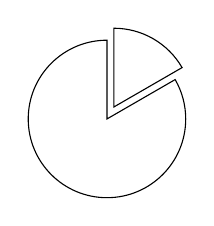
\begin{tikzpicture}
\draw(0,0)--(90:1cm)arc(90:390:1cm)--cycle;
\draw(60:5pt)--+(30:1cm)arc(30:90:1cm)--cycle;
\end{tikzpicture}


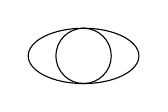
\begin{tikzpicture}
\draw (0,0) circle (10pt);
\draw (0,0) ellipse (20pt and 10pt);
\end{tikzpicture}

TikZ绘图的基本单元:路径

路径的基本元素:点、连接方式

对路径的操作:画、填充、裁剪


UNIT:cm

TikZ and PGF\footnote{Portable Graphic Format} are TeX packages for creating graphics programmatically. TikZ is build on top of PGF and allows you to create sophisticated graphics in a rather intuitive and easy manner.TikZ and PGF are TeX packages for creating graphics programmatically. TikZ is build on top of PGF and allows you to create sophisticated graphics in a rather intuitive and easy manner.

\section{Setting up a picture}

\begin{tikzpicture}[scale=4]
\draw (0,0)--(1,2);
\end{tikzpicture}

文本

\begin{figure}
	\centering
	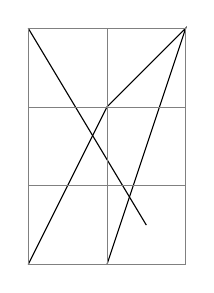
\begin{tikzpicture}
	\draw (0,0)--(1,2)--(2,3)--(1,0);
	\draw (0,3)--(1.5,0.5);
	\draw[help lines](0,0)grid(2,3);
	\end{tikzpicture}
	\caption{Captions}
\end{figure}


\subsection{Scaling pictures}
\begin{tikzpicture}[scale=3]
\draw (0,0) -- (1,1);
\end{tikzpicture}

\begin{tikzpicture}[xscale=3]
\draw (0,0) -- (1,1);
\end{tikzpicture}

\begin{tikzpicture}[xscale=2.5,yscale=0.5]
\draw (0,0) -- (1,1);
\end{tikzpicture}

\subsection{Arrows and the like}
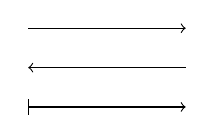
\begin{tikzpicture}
\draw [->] (0,0) -- (2,0);
\draw [<-] (0,-0.5) -- (2,-0.5);
\draw [|->] (0,-1) -- (2,-1);
\end{tikzpicture}

\begin{flushleft}
\bfseries\ttfamily{\textbackslash begin\{tikzpicture\}\\
	\textbackslash draw \verb"["<->\verb"]" (0,2)--(0,0)--(3,0);\\
	\textbackslash\{tikzpicture\}}
\end{flushleft}

\begin{tikzpicture}
\draw [<->] (0,2)--(0,0)--(3,0);
\end{tikzpicture}

\subsection{Changing the thickness of lines}
ultra thin \tikz \draw [ultra thin] (0,0)--(1,0);,\\
very thin\tikz \draw [very thin] (0,0)--(1,0);,\\
thin \tikz \draw [thin] (0,0)--(1,0);,\\
semithick \tikz \draw [semithick] (0,0)--(1,0);,\\
thick \tikz \draw [thick] (0,0)--(1,0);,\\
very thick\tikz \draw [very thick] (0,0)--(1,0);,\\
ultra thick\tikz \draw [ultra thick] (0,0)--(1,0);.

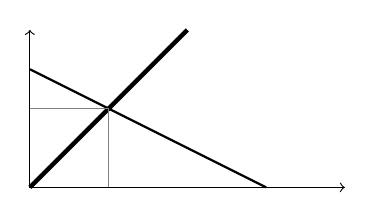
\begin{tikzpicture}
\draw [<->] (0,2) -- (0,0) -- (4,0);
\draw [thick] (0,1.5) -- (3,0);
\draw [ultra thick] (0,0) -- (2,2);
\draw [help lines] (1,0) -- (1,1) -- (0,1);
\end{tikzpicture}


\begin{tikzpicture}
\draw [line width=12] (0,0) -- (2,0);
\draw [line width=0.2cm] (4,.75) -- (5,.25);
\end{tikzpicture}

\subsection{Dashes and dots}
\begin{tikzpicture}
\draw [dashed, ultra thick] (0,1) -- (2,1);
\draw [dashed] (0, 0.5) -- (2,0.5);
\draw [dotted] (0,0) -- (2,0);
\end{tikzpicture}

\subsection{Colors}
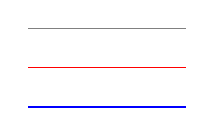
\begin{tikzpicture}
\draw [gray] (0,1) -- (2,1);
\draw [red] (0, 0.5) -- (2,0.5);
\draw [blue] (0,0) -- (2,0);
\end{tikzpicture}

red 
\begin{tikzpicture} \draw [red,line width=6](0,0)--(.5,0);\end{tikzpicture};

green \tikz \draw [green,line width=6] (0,0)--(.5,0);;

\subsection{Pictures in the middle of the text}
\subsection{Curves}
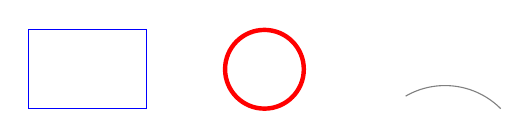
\begin{tikzpicture}
\draw [blue] (0,0) rectangle (1.5,1);
\draw [red, ultra thick] (3,0.5) circle [radius=0.5];;
\draw [gray] (6,0) arc [radius=1, start angle=45, end angle= 120];
\end{tikzpicture}

\begin{tikzpicture}
\draw [<->, rounded corners, thick, purple] (0,2) -- (0,0) -- (3,0);
\end{tikzpicture}

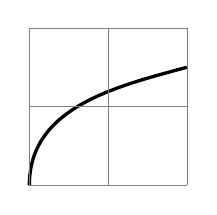
\begin{tikzpicture}
\draw[very thick] (0,0) to [out=90,in=195] (2,1.5);
\draw [help lines] (0,0)grid (2,2);
\end{tikzpicture}

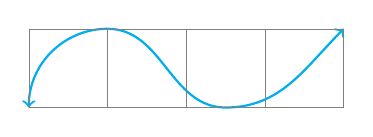
\begin{tikzpicture}
\draw [<->,thick, cyan] (0,0) to [out=90,in=180] (1,1)
to [out=0,in=180] (2.5,0) to [out=0,in=-135] (4,1) ;
\draw [help lines] (0,0)grid (4,1);
\end{tikzpicture}

\subsection{Plotting functions}
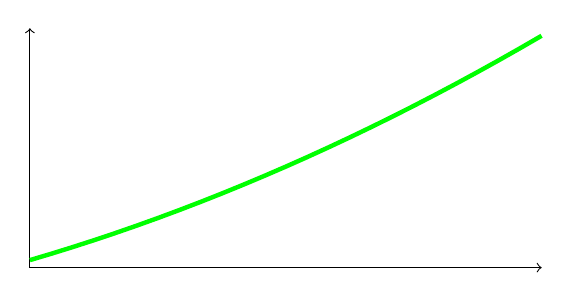
\begin{tikzpicture}[xscale=13,yscale=3.8]
\draw [<->] (0,0.8) -- (0,0) -- (0.5,0);
\draw[green, ultra thick, domain=0:0.5] plot (\x, {0.025+\x+\x*\x});
\end{tikzpicture}

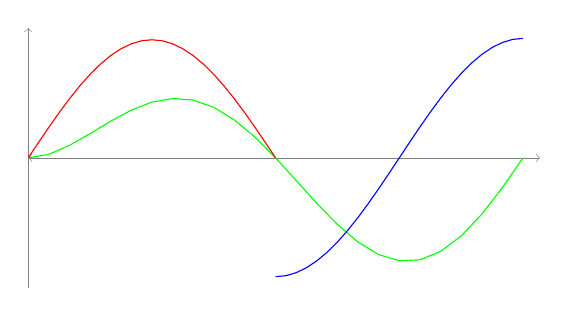
\begin{tikzpicture}[yscale=1.5]
\draw [help lines, <->] (0,0) -- (6.5,0);
\draw [help lines, ->] (0,-1.1) -- (0,1.1);
\draw [green,domain=0:2*pi] plot (\x, {(sin(\x r)* ln(\x+1))/2});
\draw [red,domain=0:pi] plot (\x, {sin(\x r)});
\draw [blue, domain=pi:2*pi] plot (\x, {cos(\x r)*exp(\x/exp(2*pi))});
\end{tikzpicture}

\section{Filling up areas}
\subsection{Filling up simple areas}
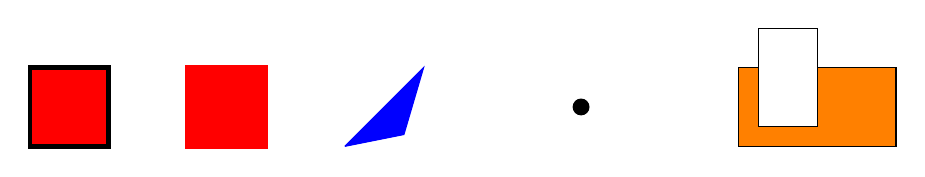
\begin{tikzpicture}
\draw [fill=red,ultra thick] (0,0) rectangle (1,1);
\draw [fill=red,ultra thick,red] (2,0) rectangle (3,1);
\draw [blue, fill=blue] (4,0) -- (5,1) -- (4.75,0.15) -- (4,0);
\draw [fill] (7,0.5) circle [radius=0.1];
\draw [fill=orange] (9,0) rectangle (11,1);
\draw [fill=white] (9.25,0.25) rectangle (10,1.5);
\end{tikzpicture}


\begin{tikzpicture}
\path [fill=gray] (0,0) rectangle (1.5,1);%没边框
\draw [fill=yellow] (2,0) rectangle (3.5,1);
\end{tikzpicture}

\subsection{Filling up arbitrary areas}

\begin{tikzpicture}
\draw [ultra thick] (0,0) to [out=87,in=150] (1,1) -- (.85,.15) -- (0,0);
\draw [ultra thick, fill=purple] (2,0) to [out=87,in=150] (3,1) -- (2.85,.15) -- (2,0);
\path [fill=purple] (4,0) to [out=87,in=150] (5,1) -- (4.85,.15) -- (4,0);
\end{tikzpicture}

\section{Putting labels in pictures}

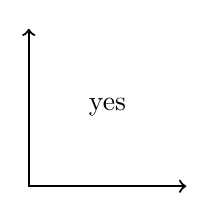
\begin{tikzpicture}
\draw [thick, <->] (0,2) -- (0,0) -- (2,0);
\node at (1,1) {yes};
\end{tikzpicture}

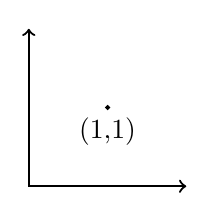
\begin{tikzpicture}
\draw [thick, <->] (0,2) -- (0,0) -- (2,0);
\draw[fill] (1,1) circle [radius=0.025];
\node [below] at (1,1) {(1,1)};
\end{tikzpicture}

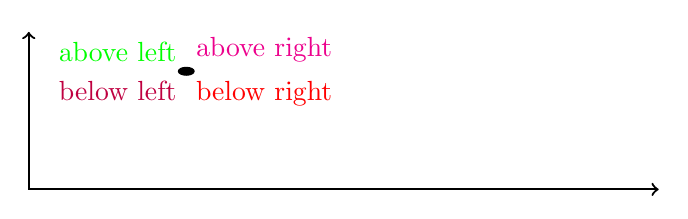
\begin{tikzpicture}[xscale=4,yscale=2]
\draw [thick, <->] (0,1) -- (0,0) -- (2,0);
\draw[fill] (.5,.75) circle [radius=0.025];
\node [below right, red] at (.5,.75) {below right};
\node [above left, green] at (.5,.75) {above left};
\node [below left, purple] at (.5,.75) {below left};
\node [above right, magenta] at (.5,.75) {above right};
\end{tikzpicture}

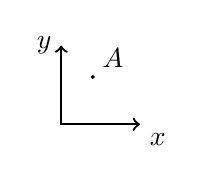
\begin{tikzpicture}
\draw [thick, <->] (0,1) -- (0,0) -- (1,0);
\node [below right] at (1,0) {$x$};
\node [left] at (0,1) {$y$};
\draw [fill] (.4,.6) circle [radius=.5pt];
\node [above right] at (.4,.6) {$A$};
\end{tikzpicture}

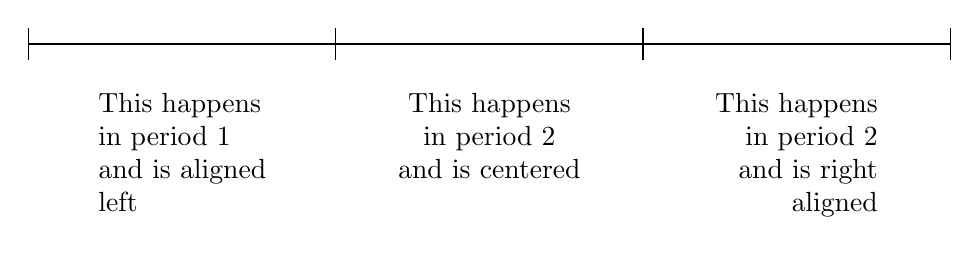
\begin{tikzpicture}[xscale=1.3]
\draw [thick] (0,0) -- (9,0);
\draw (0,-.2) -- (0, .2);
\draw (3,-.2) -- (3, .2);
\draw (6,-.2) -- (6, .2);
\draw (9,-.2) -- (9, .2);
\node[align=left, below] at (1.5,-.5)%
{This happens\\in period 1\\and is aligned\\ left};
\node[align=center, below] at (4.5,-.5)%
{This happens\\in period 2\\and is centered};
\node[align=right, below] at (7.5,-.5)%
{This happens\\in period 2\\and is right\\aligned};
\end{tikzpicture}

\section{Examples}
\subsection{Hotelling}
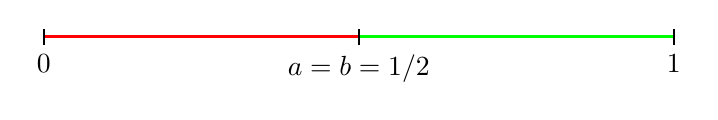
\begin{tikzpicture}[xscale=8]
\draw[-][draw=red, very thick] (0,0) -- (.5,0);
\draw[-][draw=green, very thick] (.5,0) -- (1,0);
\draw [thick] (0,-.1) node[below]{0} -- (0,0.1);
\draw [thick] (0.5,-.1) node[below]{$a=b=1/2$} -- (0.5,0.1);
\draw [thick] (1,-.1) node[below]{1} -- (1,0.1);
\end{tikzpicture}

\subsection{Vertical differentiation}
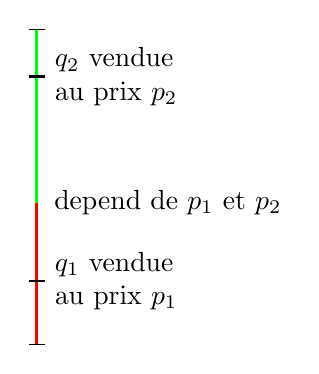
\begin{tikzpicture}[yscale=4]
\draw[-][draw=red, very thick] (0,0) -- (0,.45);
\draw[-][draw=green, very thick] (0,.45) -- (0,1);
\draw [thick] (-0.1,0.2) -- (0.1,.2) node[align=left, right]
{$q_1$ vendue\\au prix $p_1$};
\node[right] at (0.1,.45) {depend de $p_1$ et $p_2$};
\draw [thick] ((-0.1,0.85) -- (0.1,.85) node[align=left, right]
{$q_2$ vendue\\ au prix $p_2$};
\draw (-0.1,0) -- (0.1,0);
\draw (-0.1,1) -- (0.1,1);
\end{tikzpicture}

\subsection{A curve}
\begin{center}
\begin{tikzpicture}
\draw[<->] (6,0) node[below]{$q$} -- (0,0) --
(0,6) node[left]{$V(q)$};
\draw[very thick] (0,0) to [out=90,in=145] (5,4.5);
\end{tikzpicture}
\end{center}

\subsection{Tangency}
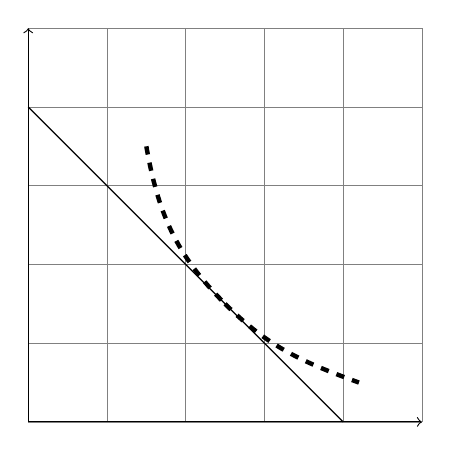
\begin{tikzpicture}
\draw [help lines] (0,0) grid (5,5);
\draw [<->] (5,0) -- (0,0) -- (0,5);
\draw (4,0) -- (0,4);
\draw[dashed,ultra thick]
(1.5,3.5) to [out=-80,in=135] (2.5,1.5);
\draw [dashed,ultra thick]
(2.5,1.5) to [out=-45,in=160] (4.2,0.5);
\end{tikzpicture}

\subsection{Consumer surplus}
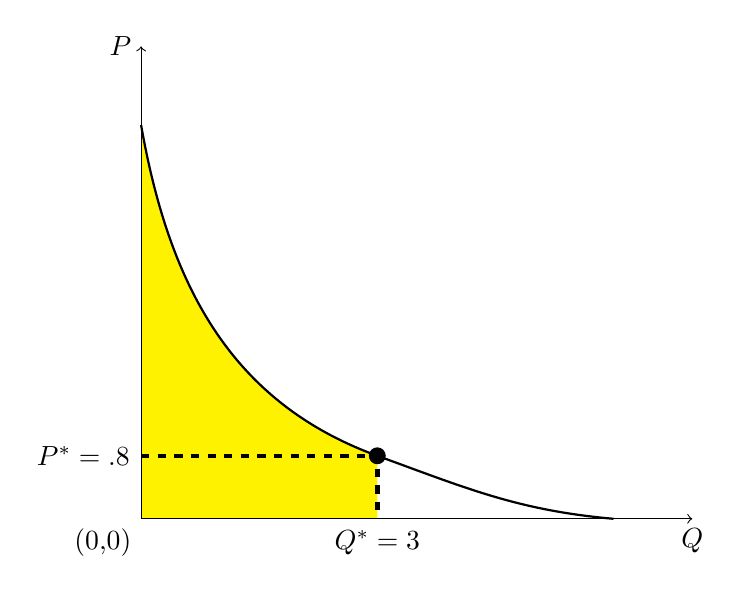
\begin{tikzpicture}
\path [fill=yellow] (0,0) -- (0,5) to [out=-80, in=160]
(3,.8) -- (3,0) -- (0,0);
\draw [<->] (0,6) node [left] {$P$} -- (0,0)
node [below left] {(0,0)} -- (7,0) node [below] {$Q$};
\draw [ultra thick, dashed] (0,.8) node [left] {$P^*=.8$} -- (3,.8)
-- (3,0) node [below] {$Q^*=3$};
\draw [fill] (3,.8) circle [radius=.1];
\draw [thick] (0,5) to [out=-80, in=160] (3,.8) to
[out=-20, in=175] (6,0);
\end{tikzpicture}

\subsection{Plotting lots of curves}
\begin{center}
	\begin{tikzpicture}[domain=0:0.5,xscale=13,yscale=3.8]
	\draw[<->] (0,2) node[left]{EUR}-- (0,0) -- (.7,0) node[below] {$q$};
	\draw[red] plot (\x, {0.25+\x/2+\x*\x/2}) node[right] {$v_1(x)$};
	\draw[green] plot (\x, {0.025+\x+\x*\x}) node[right] {$v_2(x)$};
	\draw[thin, dashed] plot (\x, {0.275+1.5*\x+1.5*\x*\x}) ;
	\draw[thick,domain=0:0.33666] plot (\x, {0.05+2*\x+2*\x*\x}) ;
	\draw[thick,domain=0.33666:0.5]
	plot (\x, {0.5+\x+\x*\x}) node[right] {$2\min[v_1,v_2]$};
	\end{tikzpicture}
\end{center}

\section{Basical shapes}
\subsection{Simple straight lines and rectangle}
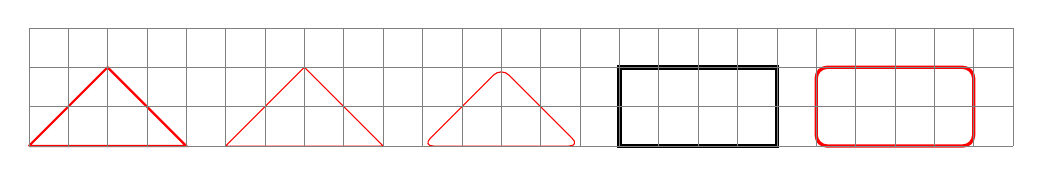
\begin{tikzpicture}[scale=0.5]
\draw [red,thick](0,0) -- (4,0)--(2,2)--(0,0);
\draw [red,](5,0)--(9,0)--(7,2)--cycle;
\draw [rounded corners,red] (10,0)--(14,0)--(12,2)--cycle;
\draw [ultra thick](15,0) rectangle (19,2);
\draw [rounded corners,red,very thick] (20,0) rectangle (24,2);
\draw [help lines] (0,0) grid (25,3);
\end{tikzpicture}

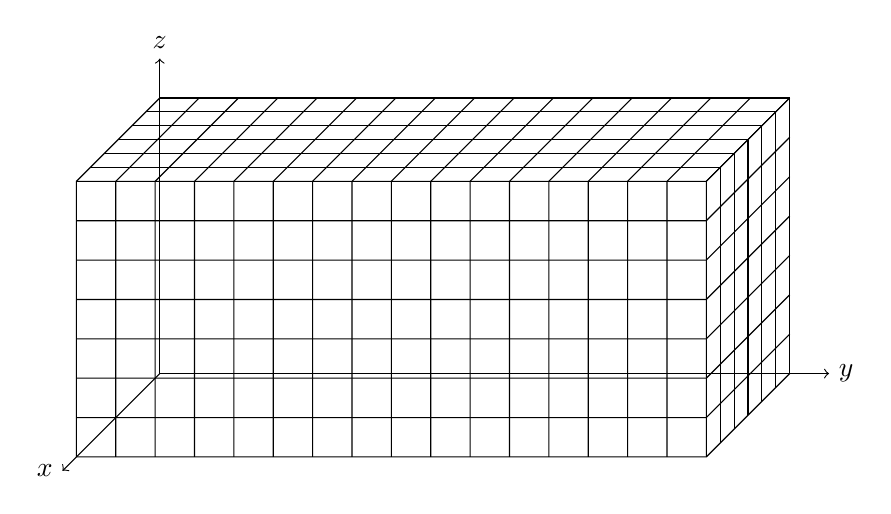
\begin{tikzpicture}[math3d,scale=0.5]
\draw[->](0,0,0)--(7,0,0)node[left]{$x$};
\draw[->](0,0,0)--(0,17,0)node[right]{$y$};
\draw[->](0,0,0)--(0,0,8)node[above]{$z$};
\foreach \z in {0,1,...,7}
\draw(6,0,\z)--(6,16,\z)--(0,16,\z);	
\foreach \y in {0,1,...,16}
\draw(6,\y,0)--(6,\y,7)--(0,\y,7);
\foreach \x in {0,1,...,6}
\draw(\x,0,7)--(\x,16,7)--(\x,16,0);	
\end{tikzpicture}

\subsection{More Examples }
\textcolor{blue}{\url{https://texample.net/tikz/examples/all/}}

\href{https://texample.net/tikz/examples/all/}{TikZ and PGF examples}


\tdplotsetmaincoords{70}{0}
\begin{tikzpicture}[tdplot_main_coords]
\def\RI{2}
\def\RII{1.25}

\draw[thick] (\RI,0)
\foreach \x in {0,300,240,180} { --  (\x:\RI) node at (\x:\RI) (R1-\x) {} };
\draw[dashed,thick] (R1-0.center)
\foreach \x in {60,120,180} { --  (\x:\RI) node at (\x:\RI) (R1-\x) {} };
\path[fill=gray!30] (\RI,0)
\foreach \x in {0,60,120,180,240,300} { --  (\x:\RI)};

\begin{scope}[yshift=2cm]
\draw[thick,fill=gray!30,opacity=0.2] (\RII,0)
\foreach \x in {0,60,120,180,240,300,360}
{ --  (\x:\RII) node at (\x:\RII) (R2-\x) {}};
\end{scope}

\foreach \x in {0,180,240,300} { \draw (R1-\x.center)--(R2-\x.center); };
\foreach \x in {60,120} { \draw[dashed] (R1-\x.center)--(R2-\x.center); };
\end{tikzpicture}

\thispagestyle{empty} 

\begin{center}
	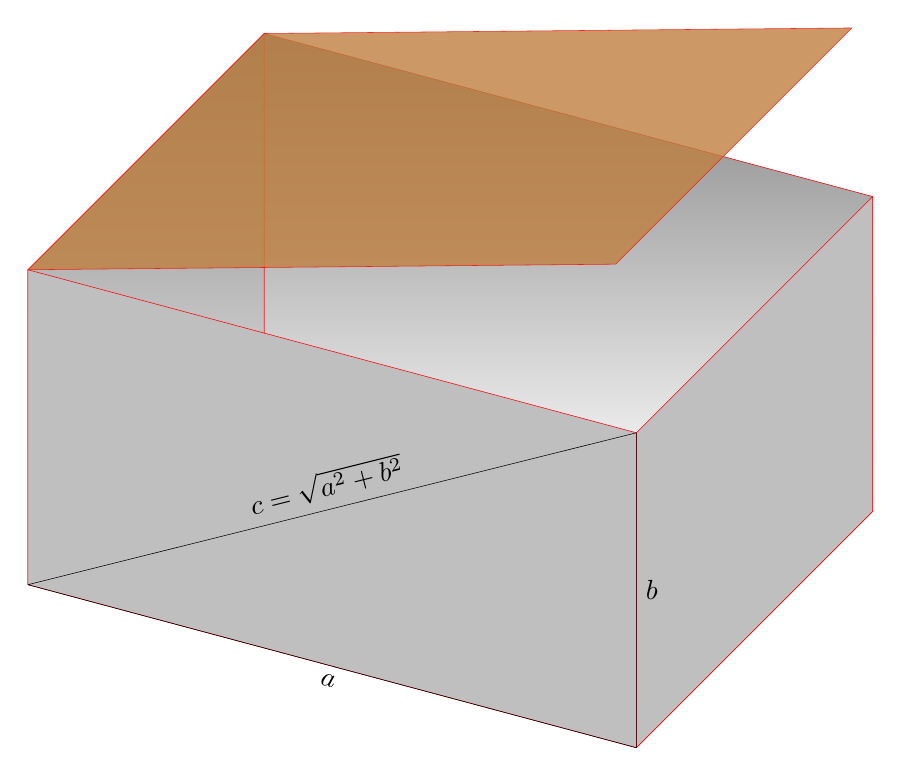
\begin{tikzpicture}[x  = {(-0.5cm,-0.5cm)},
	y  = {(0.9659cm,-0.25882cm)},
	z  = {(0cm,1cm)},
	scale = 2,
	color = {lightgray}]
	% style of faces
	\tikzset{facestyle/.style={fill=lightgray,draw=red,very thin,line join=round}}
	% face "back" 
	\begin{scope}[canvas is zy plane at x=0]
	\path[facestyle,shade] (0,0) rectangle (2,4);
	\end{scope}
	% face  "left"
	\begin{scope}[canvas is zx plane at y=0]
	\path[facestyle,shade] (0,0) rectangle (2,3);
	\end{scope}
	% face "front"
	\begin{scope}[canvas is zy plane at x=3]
	\path[facestyle] (0,0) rectangle (2,4);
	\end{scope}
	% face  "right"
	\begin{scope}[canvas is zx plane at y=4]
	\path[facestyle] (0,0) rectangle (2,3);
	\end{scope}
	% face "up" 
	\draw[fill=brown,draw=red,opacity=.8,very thin,line join=round]
	(0,0,2) -- 
	(3,0,2) --
	(3,{4*cos(15)},{4*sin(15)+2}) --
	(0,{4*cos(15)},{4*sin(15)+2}) --cycle ;
	% labels
	\draw[very thin,black,line join=round]
	(3,0,0) -- node [sloped,below] {$a$}    
	(3,4,0) -- node [right]        {$b $}
	(3,4,2) -- node [sloped,above] {$c=\sqrt{a^2+b^2}$} 
	(3,0,0);
	\end{tikzpicture}
\end{center}


\chapter{tikz-3dplot}
%\begin{tikzpicture}[%
%x={(\raarot cm,\rbarot cm)},%
%y={(\rabrot cm, \rbbrot cm)},%
%z={(\racrot, \rbcrot cm)}]

\section{矩阵变换}

\section{Styles}
\begin{itemize}
	\item tdplot\_main\_coords
	\item tdplot\_rotated\_coords
	\item tdplot\_screen\_coords
\end{itemize}

\section{Commands}
\begin{verbatim}
\tdplotsetmaincoords{\theta_d}{\phi_d} % 顺时针方向转?!
\end{verbatim}

\qd{Example 1}

\begin{verbatim}
\tdplotsetmaincoords{70}{110} %'td' means 'three dimention';
\begin{tikzpicture}[tdplot_main_coords]
\draw[thick,->] (0,0,0) -- (1,0,0) node[anchor=north east]{$x$};
\draw[thick,->] (0,0,0) -- (0,1,0) node[anchor=north west]{$y$};
\draw[thick,->] (0,0,0) -- (0,0,1) node[anchor=south]{$z$};
\end{tikzpicture}
\end{verbatim}


\tdplotsetmaincoords{70}{110}
\begin{tikzpicture}[tdplot_main_coords,scale=4]
\draw[thick,->] (0,0,0) -- (1,0,0) node[anchor=north east]{$x$};
\draw[thick,->] (0,0,0) -- (0,1,0) node[anchor=north west]{$y$};
\draw[thick,->] (0,0,0) -- (0,0,1) node[anchor=south]{$z$};
\end{tikzpicture}


\qd{Example 2}
\begin{verbatim}
\tdplotsetrotatedcoords{\alpha}{\beta}{\gamma}
\end{verbatim}

\begin{verbatim}
\tdplotsetmaincoords{70}{110}
\begin{tikzpicture}[tdplot_main_coords]
\draw[thick,->] (0,0,0) -- (1,0,0) node[anchor=north east]{$x$};
\draw[thick,->] (0,0,0) -- (0,1,0) node[anchor=north west]{$y$};
\draw[thick,->] (0,0,0) -- (0,0,1) node[anchor=south]{$z$};

\tdplotsetrotatedcoords{60}{40}{30}
\draw[thick,color=blue,tdplot_rotated_coords,->] (0,0,0) --
(.7,0,0) node[anchor=north]{$x’$};
\draw[thick,color=blue,tdplot_rotated_coords,->] (0,0,0) --
(0,.7,0) node[anchor=west]{$y’$};
\draw[thick,color=blue,tdplot_rotated_coords,->] (0,0,0) --
(0,0,.7) node[anchor=south]{$z’$};
\end{tikzpicture}
\end{verbatim}

\tdplotsetmaincoords{70}{110}
\begin{tikzpicture}[tdplot_main_coords,scale=5]
\draw[thick,->] (0,0,0) -- (1,0,0) node[anchor=north east]{$x$};
\draw[thick,->] (0,0,0) -- (0,1,0) node[anchor=north west]{$y$};
\draw[thick,->] (0,0,0) -- (0,0,1) node[anchor=south]{$z$};

\tdplotsetrotatedcoords{60}{20}{30}
\draw[thick,color=blue,tdplot_rotated_coords,->] (0,0,0) --
(.7,0,0) node[anchor=north]{$x’$};
\draw[thick,color=blue,tdplot_rotated_coords,->] (0,0,0) --
(0,.7,0) node[anchor=west]{$y’$};
\draw[thick,color=blue,tdplot_rotated_coords,->] (0,0,0) --
(0,0,.7) node[anchor=south]{$z’$};
\end{tikzpicture}

\qd{Example 3}

\begin{verbatim}
\tdplotsetrotatedcoordsorigin{point} % 设置原点
\tdplotresetrotatedcoordsorigin  %重置原点
\end{verbatim}

\begin{verbatim}
\tdplotsetmaincoords{70}{110}
\begin{tikzpicture}[tdplot_main_coords]
\draw[thick,->] (0,0,0) -- (1,0,0) node[anchor=north east]{$x$};
\draw[thick,->] (0,0,0) -- (0,1,0) node[anchor=north west]{$y$};
\draw[thick,->] (0,0,0) -- (0,0,1) node[anchor=south]{$z$};
\tdplotsetrotatedcoords{60}{40}{30}
\coordinate (Shift) at (0.5,0.5,0.5);
\tdplotsetrotatedcoordsorigin{(Shift)}
\draw[thick,color=blue,tdplot_rotated_coords,->] (0,0,0) --
(.7,0,0) node[anchor=north]{$x’$};
\draw[thick,color=blue,tdplot_rotated_coords,->] (0,0,0) --
(0,.7,0) node[anchor=west]{$y’$};
\draw[thick,color=blue,tdplot_rotated_coords,->] (0,0,0) --
(0,0,.7) node[anchor=south]{$z’$};
\end{tikzpicture}
\end{verbatim}

\tdplotsetmaincoords{70}{110}
\begin{tikzpicture}[tdplot_main_coords,scale=5]
\draw[thick,->] (0,0,0) -- (1,0,0) node[anchor=north east]{$x$};
\draw[thick,->] (0,0,0) -- (0,1,0) node[anchor=north west]{$y$};
\draw[thick,->] (0,0,0) -- (0,0,1) node[anchor=south]{$z$};
\tdplotsetrotatedcoords{60}{20}{30}
\coordinate (Shift) at (0.5,0.5,0.5);
\tdplotsetrotatedcoordsorigin{(Shift)}
\draw[thick,color=blue,tdplot_rotated_coords,->] (0,0,0) --
(.7,0,0) node[anchor=north]{$x^\prime$};
\draw[thick,color=blue,tdplot_rotated_coords,->] (0,0,0) --
(0,.7,0) node[anchor=west]{$y^\prime$};
\draw[thick,color=blue,tdplot_rotated_coords,->] (0,0,0) --
(0,0,.7) node[anchor=south]{$z^\prime$};
\end{tikzpicture}

\qd{Example}

\begin{verbatim}
\tdplotsetthetaplanecoords{\phi} % theta plane; 一种建立旋转坐标系的新方法;
% 注意是x'y'与xz的夹角。
\end{verbatim}

\begin{verbatim}
\tdplotsetmaincoords{70}{110}
\begin{tikzpicture}[scale=3,tdplot_main_coords,scale=5]
\draw[thick,->] (0,0,0) -- (1,0,0) node[anchor=north east]{$x$};
\draw[thick,->] (0,0,0) -- (0,1,0) node[anchor=north west]{$y$};
\draw[thick,->] (0,0,0) -- (0,0,1) node[anchor=south]{$z$};
\tdplotsetcoord{P}{.8}{50}{70}
%draw a vector from origin to point (P)
\draw[-stealth,color=red] (O) -- (P);
%draw projection on xy plane, and a connecting line
\draw[dashed, color=red] (O) -- (Pxy);
\draw[dashed, color=red] (P) -- (Pxy);
\tdplotsetthetaplanecoords{70}
\draw[tdplot_rotated_coords,color=blue,thick,->] (0,0,0)
-- (.2,0,0) node[anchor=east]{$x’$};
\draw[tdplot_rotated_coords,color=blue,thick,->] (0,0,0)
-- (0,.2,0) node[anchor=north]{$y’$};
\draw[tdplot_rotated_coords,color=blue,thick,->] (0,0,0)
-- (0,0,.2) node[anchor=west]{$z’$};
\end{tikzpicture}
\end{verbatim}

\tdplotsetmaincoords{70}{110}
\begin{tikzpicture}[scale=6,tdplot_main_coords]
\draw[thick,->] (0,0,0) -- (1,0,0) node[anchor=north east]{$x$};
\draw[thick,->] (0,0,0) -- (0,1,0) node[anchor=north west]{$y$};
\draw[thick,->] (0,0,0) -- (0,0,1) node[anchor=south]{$z$};
\tdplotsetcoord{O}{0}{0}{0}
\tdplotsetcoord{P}{.8}{50}{50}
%draw a vector from origin to point (P)
\draw[-stealth,color=red] (O) -- (P);
%draw projection on xy plane, and a connecting line
\draw[dashed, color=red] (O) -- (Pxy);
\draw[dashed, color=red] (P) -- (Pxy);
\tdplotsetthetaplanecoords{180}
%\tdplotsetrotatedcoords{50}{0}{0}
\draw[tdplot_rotated_coords,color=blue,thick,->] (0,0,0)
-- (.9,0,0) node[anchor=east]{$x^\prime$};
\draw[tdplot_rotated_coords,color=blue,thick,->] (0,0,0)
-- (0,.9,0) node[anchor=north]{$y^\prime$};
\draw[tdplot_rotated_coords,color=blue,thick,->] (0,0,0)
-- (0,0,.9) node[anchor=west]{$z^\prime$};


\end{tikzpicture}

\qd{Example}

\begin{verbatim}
tdplotsetrotatedthetaplanecoords{\phi^\prime} %与旋转坐标系的夹角!
\end{verbatim}

\begin{verbatim}
\tdplotsetmaincoords{60}{110}
\begin{tikzpicture}[scale=3,tdplot_main_coords]
\draw[thick,->] (0,0,0) -- (1,0,0) node[anchor=north east]{$x$};
\draw[thick,->] (0,0,0) -- (0,1,0) node[anchor=north west]{$y$};
\draw[thick,->] (0,0,0) -- (0,0,1) node[anchor=south]{$z$};
\coordinate (Shift) at (2,2,2);
\tdplotsetrotatedcoords{-20}{10}{0}
\tdplotsetrotatedcoordsorigin{(Shift)}
\draw[thick,color=blue,tdplot_rotated_coords,->] (0,0,0)
-- (1,0,0) node[anchor=south east]{$x’$};
\draw[thick,color=blue,tdplot_rotated_coords,->] (0,0,0)
-- (0,1,0) node[anchor=west]{$y’$};
\draw[thick,color=blue,tdplot_rotated_coords,->] (0,0,0)
-- (0,0,1) node[anchor=south]{$z’$};
\tdplotsetrotatedthetaplanecoords{30}
\draw[thick,color=blue,tdplot_rotated_coords,->] (0,0,0)
-- (.5,0,0) node[anchor=south east]{$x’’$};
\draw[thick,color=blue,tdplot_rotated_coords,->] (0,0,0)
-- (0,.5,0) node[anchor=west]{$y’’$};
\draw[thick,color=blue,tdplot_rotated_coords,->] (0,0,0)
-- (0,0,.5) node[anchor=south]{$z’’$};
\end{tikzpicture}
\end{verbatim}

\tdplotsetmaincoords{60}{110}
\begin{tikzpicture}[scale=7,tdplot_main_coords]
\draw[thick,->] (0,0,0) -- (1,0,0) node[anchor=north east]{$x$};
\draw[thick,->] (0,0,0) -- (0,1,0) node[anchor=north west]{$y$};
\draw[thick,->] (0,0,0) -- (0,0,1) node[anchor=south]{$z$};
\coordinate (Shift) at (2,2,2);
\tdplotsetrotatedcoords{-20}{10}{0}
\tdplotsetrotatedcoordsorigin{(Shift)}
\draw[thick,color=blue,tdplot_rotated_coords,->] (0,0,0)
-- (1,0,0) node[anchor=south east]{$x^\prime$};
\draw[thick,color=blue,tdplot_rotated_coords,->] (0,0,0)
-- (0,1,0) node[anchor=west]{$y^\prime$};
\draw[thick,color=blue,tdplot_rotated_coords,->] (0,0,0)
-- (0,0,1) node[anchor=south]{$z^\prime$};
\tdplotsetrotatedthetaplanecoords{30}
\draw[thick,color=blue,tdplot_rotated_coords,->] (0,0,0)
-- (.5,0,0) node[anchor=south east]{$x^{\prime\prime}$};
\draw[thick,color=blue,tdplot_rotated_coords,->] (0,0,0)
-- (0,.5,0) node[anchor=west]{$y^{\prime\prime}$};
\draw[thick,color=blue,tdplot_rotated_coords,->] (0,0,0)
-- (0,0,.5) node[anchor=south]{$z^{\prime\prime}$};
\end{tikzpicture}

\qd{计算转换矩阵}

\begin{verbatim}
\tdplotcalctransformmainrot
\tdplotcalctransformrotmain
\tdplotcalctransformmainscreen
\end{verbatim}

\subsection{Point calculation commands}

\begin{verbatim}
\tdplotsetcoord{point}{r}{θ}{φ}
\end{verbatim}

\begin{verbatim}
\tdplotsetmaincoords{60}{130}
\begin{tikzpicture}[scale=2,tdplot_main_coords]
\coordinate (O) at (0,0,0);
\tdplotsetcoord{P}{.8}{55}{60} % 产生点坐标:\tdplotsetcoord{point}{r}{θ}{φ}
\draw[thick,->] (0,0,0) -- (1,0,0) node[anchor=north east]{$x$};
\draw[thick,->] (0,0,0) -- (0,1,0) node[anchor=north west]{$y$};
\draw[thick,->] (0,0,0) -- (0,0,1) node[anchor=south]{$z$};
\draw[-stealth,color=red] (O) -- (P);
\draw[dashed, color=red] (O) -- (Px);
\draw[dashed, color=red] (O) -- (Py);
\draw[dashed, color=red] (O) -- (Pz);
\draw[dashed, color=red] (Px) -- (Pxy);
\draw[dashed, color=red] (Py) -- (Pxy);
\draw[dashed, color=red] (Px) -- (Pxz);
\draw[dashed, color=red] (Pz) -- (Pxz);
\draw[dashed, color=red] (Py) -- (Pyz);
\draw[dashed, color=red] (Pz) -- (Pyz);
\draw[dashed, color=red] (Pxy) -- (P);
\draw[dashed, color=red] (Pxz) -- (P);
\draw[dashed, color=red] (Pyz) -- (P);
\end{tikzpicture}
\end{verbatim}

\tdplotsetmaincoords{60}{130}
\begin{tikzpicture}[scale=6,tdplot_main_coords]
\coordinate (O) at (0,0,0);
\tdplotsetcoord{P}{.8}{55}{60}
\draw[thick,->] (0,0,0) -- (1,0,0) node[anchor=north east]{$x$};
\draw[thick,->] (0,0,0) -- (0,1,0) node[anchor=north west]{$y$};
\draw[thick,->] (0,0,0) -- (0,0,1) node[anchor=south]{$z$};
\draw[-stealth,color=red] (O) -- (P);
\draw[dashed, color=red] (O) -- (Px);
\draw[dashed, color=red] (O) -- (Py);
\draw[dashed, color=red] (O) -- (Pz);
\draw[dashed, color=red] (Px) -- (Pxy);
\draw[dashed, color=red] (Py) -- (Pxy);
\draw[dashed, color=red] (Px) -- (Pxz);
\draw[dashed, color=red] (Pz) -- (Pxz);
\draw[dashed, color=red] (Py) -- (Pyz);
\draw[dashed, color=red] (Pz) -- (Pyz);
\draw[dashed, color=red] (Pxy) -- (P);
\draw[dashed, color=red] (Pxz) -- (P);
\draw[dashed, color=red] (Pyz) -- (P);
\end{tikzpicture}

\begin{verbatim}
\tdplotsetmaincoords{50}{140}
\begin{tikzpicture}[scale=2,tdplot_main_coords]
\draw[thick,->] (0,0,0) -- (1,0,0) node[anchor=north east]{$x$};
\draw[thick,->] (0,0,0) -- (0,1,0) node[anchor=north west]{$y$};
\draw[thick,->] (0,0,0) -- (0,0,1) node[anchor=south]{$z$};
\pgfmathsetmacro{\ax}{2}
\pgfmathsetmacro{\ay}{2}
\pgfmathsetmacro{\az}{1}
\tdplotsetrotatedcoords{20}{40}{00}
\draw[thick,color=red,tdplot_rotated_coords,->] (0,0,0)
-- (.7,0,0) node[anchor=east]{$x’$};
\draw[thick,color=green!50!black,tdplot_rotated_coords,->] (0,0,0)
-- (0,.7,0) node[anchor=west]{$y’$};
\draw[thick,color=blue,tdplot_rotated_coords,->] (0,0,0)
-- (0,0,.7) node[anchor=south]{$z’$};
\tdplottransformmainrot{\ax}{\ay}{\az} 
% 坐标转换:\tdplottransformmainrot{x}{y}{z}
\draw[tdplot_rotated_coords,->,blue!50] (0,0,0)
-- (\tdplotresx,\tdplotresy,\tdplotresz);
\node[tdplot_main_coords,anchor=south]
at (\ax,\ay,\az){Main coords: (\ax, \ay, \az)};
\node[tdplot_rotated_coords,anchor=north]
at (\tdplotresx,\tdplotresy,\tdplotresz)
{Rotated coords: (\tdplotresx, \tdplotresy, \tdplotresz)}; 
% 转换后的坐标: (\tdplotresx, \tdplotresy, \tdplotresz)
\end{tikzpicture}
\end{verbatim}

\tdplotsetmaincoords{50}{140}
\begin{tikzpicture}[scale=5,tdplot_main_coords]
\draw[thick,->] (0,0,0) -- (1,0,0) node[anchor=north east]{$x$};
\draw[thick,->] (0,0,0) -- (0,1,0) node[anchor=north west]{$y$};
\draw[thick,->] (0,0,0) -- (0,0,1) node[anchor=south]{$z$};
\pgfmathsetmacro{\ax}{2}
\pgfmathsetmacro{\ay}{2}
\pgfmathsetmacro{\az}{1}
\tdplotsetrotatedcoords{20}{40}{00}
\draw[thick,color=red,tdplot_rotated_coords,->] (0,0,0)
-- (.7,0,0) node[anchor=east]{$x^\prime$};
\draw[thick,color=green!50!black,tdplot_rotated_coords,->] (0,0,0)
-- (0,.7,0) node[anchor=west]{$y^\prime$};
\draw[thick,color=blue,tdplot_rotated_coords,->] (0,0,0)
-- (0,0,.7) node[anchor=south]{$z^\prime$};
\tdplottransformmainrot{\ax}{\ay}{\az}
\draw[tdplot_rotated_coords,->,blue!50] (0,0,0)
-- (\tdplotresx,\tdplotresy,\tdplotresz);
\node[tdplot_main_coords,anchor=south]
at (\ax,\ay,\az){Main coords: (\ax, \ay, \az)};
\node[tdplot_rotated_coords,anchor=north]
at (\tdplotresx,\tdplotresy,\tdplotresz)
{Rotated coords: (\tdplotresx, \tdplotresy, \tdplotresz)};
\end{tikzpicture}


\begin{verbatim}
\tdplotsetmaincoords{50}{140}
\begin{tikzpicture}[scale=2,tdplot_main_coords]
\draw[thick,->] (0,0,0) -- (1,0,0) node[anchor=north east]{$x$};
\draw[thick,->] (0,0,0) -- (0,1,0) node[anchor=north west]{$y$};
\draw[thick,->] (0,0,0) -- (0,0,1) node[anchor=south]{$z$};
\pgfmathsetmacro{\ax}{-.75}
\pgfmathsetmacro{\ay}{2.5}
\pgfmathsetmacro{\az}{0}
\tdplotsetrotatedcoords{20}{40}{00}
\draw[thick,color=red,tdplot_rotated_coords,->] (0,0,0)
-- (.7,0,0) node[anchor=east]{$x’$};
\draw[thick,color=green!50!black,tdplot_rotated_coords,->] (0,0,0)
-- (0,.7,0) node[anchor=west]{$y’$};
\draw[thick,color=blue,tdplot_rotated_coords,->] (0,0,0)
-- (0,0,.7) node[anchor=south]{$z’$};
\tdplottransformrotmain{\ax}{\ay}{\az}
% 坐标转换:\tdplottransformrotmain{x}{y}{z}
\draw[tdplot_main_coords,->,blue!50] (0,0,0)
-- (\tdplotresx,\tdplotresy,\tdplotresz);
\node[tdplot_rotated_coords,anchor=north]
at (\ax,\ay,\az){Rotated coords: (\ax, \ay, \az)};
\node[tdplot_main_coords,anchor=south]
at (\tdplotresx,\tdplotresy,\tdplotresz)
{Main coords: (\tdplotresx, \tdplotresy, \tdplotresz)};
% 转换后的坐标: (\tdplotresx, \tdplotresy, \tdplotresz)
\end{tikzpicture}
\end{verbatim}

\tdplotsetmaincoords{50}{140}
\begin{tikzpicture}[scale=5,tdplot_main_coords]
\draw[thick,->] (0,0,0) -- (1,0,0) node[anchor=north east]{$x$};
\draw[thick,->] (0,0,0) -- (0,1,0) node[anchor=north west]{$y$};
\draw[thick,->] (0,0,0) -- (0,0,1) node[anchor=south]{$z$};
\pgfmathsetmacro{\ax}{-.75}
\pgfmathsetmacro{\ay}{2.5}
\pgfmathsetmacro{\az}{0}
\tdplotsetrotatedcoords{20}{40}{00}
\draw[thick,color=red,tdplot_rotated_coords,->] (0,0,0)
-- (.7,0,0) node[anchor=east]{$x’$};
\draw[thick,color=green!50!black,tdplot_rotated_coords,->] (0,0,0)
-- (0,.7,0) node[anchor=west]{$y’$};
\draw[thick,color=blue,tdplot_rotated_coords,->] (0,0,0)
-- (0,0,.7) node[anchor=south]{$z’$};
\tdplottransformrotmain{\ax}{\ay}{\az}
\draw[tdplot_main_coords,->,blue!50] (0,0,0)
-- (\tdplotresx,\tdplotresy,\tdplotresz);
\node[tdplot_rotated_coords,anchor=north]
at (\ax,\ay,\az){Rotated coords: (\ax, \ay, \az)};
\node[tdplot_main_coords,anchor=south]
at (\tdplotresx,\tdplotresy,\tdplotresz)
{Main coords: (\tdplotresx, \tdplotresy, \tdplotresz)};
\end{tikzpicture}

\begin{verbatim}
\tdplotsetmaincoords{50}{140}
\begin{tikzpicture}[scale=2,tdplot_main_coords]
\draw[thick,->] (0,0,0) -- (1,0,0) node[anchor=north east]{$x$};
\draw[thick,->] (0,0,0) -- (0,1,0) node[anchor=north west]{$y$};
\draw[thick,->] (0,0,0) -- (0,0,1) node[anchor=south]{$z$};
\pgfmathsetmacro{\ax}{2}
\pgfmathsetmacro{\ay}{3}
\pgfmathsetmacro{\az}{1}
\tdplottransformmainscreen{\ax}{\ay}{\az}
% \tdplottransformmainscreen{x}{y}{z}
\draw[tdplot_screen_coords,->,blue!50] (0,0)
-- (\tdplotresx,\tdplotresy);
\node[tdplot_main_coords,anchor=south]
at (\ax,\ay,\az){Main coords: (\ax, \ay, \az)};
\node[tdplot_screen_coords,anchor=north]
at (\tdplotresx,\tdplotresy)
{Screen coords: (\tdplotresx, \tdplotresy)};
% 转换后的坐标: (\tdplotresx, \tdplotresy)
\end{tikzpicture}
\end{verbatim}


\tdplotsetmaincoords{50}{140}
\begin{tikzpicture}[scale=5,tdplot_main_coords]
\draw[thick,->] (0,0,0) -- (1,0,0) node[anchor=north east]{$x$};
\draw[thick,->] (0,0,0) -- (0,1,0) node[anchor=north west]{$y$};
\draw[thick,->] (0,0,0) -- (0,0,1) node[anchor=south]{$z$};
\pgfmathsetmacro{\ax}{2}
\pgfmathsetmacro{\ay}{3}
\pgfmathsetmacro{\az}{1}
\tdplottransformmainscreen{\ax}{\ay}{\az}
% \tdplottransformmainscreen{x}{y}{z}
\draw[tdplot_screen_coords,->,blue!50] (0,0)
-- (\tdplotresx,\tdplotresy);
\node[tdplot_main_coords,anchor=south]
at (\ax,\ay,\az){Main coords: (\ax, \ay, \az)};
\node[tdplot_screen_coords,anchor=north]
at (\tdplotresx,\tdplotresy)
{Screen coords: (\tdplotresx, \tdplotresy)};
% 转换后的坐标: (\tdplotresx, \tdplotresy)
\end{tikzpicture}

\newpage

\begin{verbatim}
\tdplotsetmaincoords{60}{110}%
\pgfmathsetmacro{\rvec}{.8}
\pgfmathsetmacro{\thetavec}{30}
\pgfmathsetmacro{\phivec}{60}
%
\begin{tikzpicture}[scale=5,tdplot_main_coords]
\coordinate (O) at (0,0,0); 
\draw[thick,->] (0,0,0) -- (1,0,0) node[anchor=north east]{$x$}; 
\draw[thick,->] (0,0,0) -- (0,1,0) node[anchor=north west]{$y$};
\draw[thick,->] (0,0,0) -- (0,0,1) node[anchor=south]{$z$}; \draw[thick,->] (0,0,0) -- (0,0,1) node[anchor=south]{$z$};
\tdplotsetcoord{P}{\rvec}{\thetavec}{\phivec}
\draw[-stealth,color=red] (O) -- (P);
\draw[dashed, color=red] (O) -- (Pxy);
\draw[dashed, color=red] (P) -- (Pxy);
\tdplotdrawarc{(O)}{0.2}{0}{\phivec}{anchor=north}{$\phi$}
\tdplotsetthetaplanecoords{\phivec}
\tdplotdrawarc[tdplot_rotated_coords]{(0,0,0)}{0.5}{0}%
{\thetavec}{anchor=south west}{$\theta$}
\draw[dashed,tdplot_rotated_coords] (\rvec,0,0) arc (0:90:\rvec);
\draw[dashed] (\rvec,0,0) arc (0:90:\rvec);
\tdplotsetrotatedcoords{\phivec}{\thetavec}{0}
\tdplotsetrotatedcoordsorigin{(P)}
\draw[thick,tdplot_rotated_coords,->] (0,0,0)
-- (.5,0,0) node[anchor=north west]{$x^\prime$};
\draw[thick,tdplot_rotated_coords,->] (0,0,0)
-- (0,.5,0) node[anchor=west]{$y^\prime$};
\draw[thick,tdplot_rotated_coords,->] (0,0,0)
-- (0,0,.5) node[anchor=south]{$z^\prime$};
\draw[-stealth,color=blue,tdplot_rotated_coords] (0,0,0) -- (.2,.2,.2);
\draw[dashed,color=blue,tdplot_rotated_coords] (0,0,0) -- (.2,.2,0);
\draw[dashed,color=blue,tdplot_rotated_coords] (.2,.2,0) -- (.2,.2,.2);
\tdplotdrawarc[tdplot_rotated_coords,color=blue]{(0,0,0)}{0.2}{0}%
{45}{anchor=north west,color=black}{$\phi^\prime$}
\tdplotsetrotatedthetaplanecoords{45}
\tdplotdrawarc[tdplot_rotated_coords,color=blue]{(0,0,0)}{0.2}{0}%
{55}{anchor=south west,color=black}{$\theta^\prime$}
\end{verbatim}


\tdplotsetmaincoords{60}{110}%
\pgfmathsetmacro{\rvec}{.8}
\pgfmathsetmacro{\thetavec}{30}
\pgfmathsetmacro{\phivec}{60}
%

\begin{center}
	\begin{figure}
\begin{tikzpicture}[scale=7,tdplot_main_coords]
\coordinate (O) at (0,0,0); 
\draw[thick,->] (0,0,0) -- (1,0,0) node[anchor=north east]{$x$}; 
\draw[thick,->] (0,0,0) -- (0,1,0) node[anchor=north west]{$y$};
\draw[thick,->] (0,0,0) -- (0,0,1) node[anchor=south]{$z$};
\tdplotsetcoord{P}{\rvec}{\thetavec}{\phivec}
\draw[-stealth,color=red] (O) -- (P);
\draw[dashed, color=red] (O) -- (Pxy);
\draw[dashed, color=red] (P) -- (Pxy);
\tdplotdrawarc{(O)}{0.2}{0}{\phivec}{anchor=north}{$\phi$}
\tdplotsetthetaplanecoords{\phivec}
\tdplotdrawarc[tdplot_rotated_coords]{(0,0,0)}{0.5}{0}%
{\thetavec}{anchor=south west}{$\theta$}
\draw[dashed,tdplot_rotated_coords] (\rvec,0,0) arc (0:90:\rvec);
\draw[dashed] (\rvec,0,0) arc (0:90:\rvec);
\tdplotsetrotatedcoords{\phivec}{\thetavec}{0}
\tdplotsetrotatedcoordsorigin{(P)}
\draw[thick,tdplot_rotated_coords,->] (0,0,0)
-- (.5,0,0) node[anchor=north west]{$x^\prime$};
\draw[thick,tdplot_rotated_coords,->] (0,0,0)
-- (0,.5,0) node[anchor=west]{$y^\prime$};
\draw[thick,tdplot_rotated_coords,->] (0,0,0)
-- (0,0,.5) node[anchor=south]{$z^\prime$};
\draw[-stealth,color=blue,tdplot_rotated_coords] (0,0,0) -- (.2,.2,.2);
\draw[dashed,color=blue,tdplot_rotated_coords] (0,0,0) -- (.2,.2,0);
\draw[dashed,color=blue,tdplot_rotated_coords] (.2,.2,0) -- (.2,.2,.2);
\tdplotdrawarc[tdplot_rotated_coords,color=blue]{(0,0,0)}{0.2}{0}%
{45}{anchor=north west,color=black}{$\phi^\prime$}
\tdplotsetrotatedthetaplanecoords{45}
\tdplotdrawarc[tdplot_rotated_coords,color=blue]{(0,0,0)}{0.2}{0}%
{55}{anchor=south west,color=black}{$\theta^\prime$}
\end{tikzpicture}
\end{figure}
\end{center}


\chapter{TackChanges}

\chapter{Asymptote}



\end{document}